\documentclass[12pt,a4paper]{report}
\usepackage{geometry}
\geometry{hmargin=2.5cm,vmargin=1.5cm}
\usepackage[utf8]{inputenc}
\usepackage[francais]{babel}
\usepackage[T1]{fontenc}
\usepackage{amsmath}
\usepackage{amsfonts}
\usepackage{amssymb}
\usepackage{graphicx}
\usepackage{lmodern}
\usepackage{xcolor}
\usepackage{cover}
\usepackage{fancyhdr}
\usepackage[final]{pdfpages}
\usepackage{eurosym}
\usepackage{listings}
\usepackage{upquote}
\lstset{
language=Java,
basicstyle=\scriptsize, % ou ça==> basicstyle=\scriptsize,
upquote=true,
aboveskip={1.5\baselineskip},
columns=fullflexible,
showstringspaces=false,
extendedchars=true,
breaklines=true,
showtabs=false,
showspaces=false,
showstringspaces=false,
identifierstyle=\ttfamily,
keywordstyle=\color[rgb]{0,0,1},
commentstyle=\color[rgb]{0.133,0.545,0.133},
stringstyle=\color[rgb]{0.627,0.126,0.941},
numbers=left ,
numberstyle=\tiny\bfseries\underline ,
stepnumber=1,
firstnumber=1,
numberfirstline=true
language={java}
}

\usepackage{caption}
\DeclareCaptionFont{white}{\color{white}}
\DeclareCaptionFormat{listing}{\colorbox{gray}{\parbox{\textwidth}{#1#2#3}}}
\captionsetup[lstlisting]{format=listing,labelfont=white,textfont=white}

\pagestyle{fancy}
\lhead{Pierrick CHOVELON - Julien TIRON}
\rhead{INF 112}

%%%% debut macro %%%%
\makeatletter
\renewcommand{\fnum@figure}{\small\textbf{\figurename~\thefigure}}
\renewcommand{\fnum@table}{\small\textbf{\tablename~\thetable}}
\makeatother
%%%% fin macro %%%%


\renewcommand{\familydefault}{\sfdefault} 
%\renewcommand{\scdefault}{\sfdefault} 

\definecolor{VertClair}{cmyk}{0.4,0.1,1,0}
\definecolor{VertFonce}{cmyk}{1,0.55,0.5,0.5}
% \makeatletter
% \renewcommand\section{\@startsection {section}{1}{\z@}%
%                                    {-3.5ex \@plus -1ex \@minus -.2ex}%
%                                    {2.3ex \@plus.2ex}%
%                                    {\normalfont\Large\bfseries\color{VertClair}}}
%\parskip=3pt

\renewcommand{\chaptername}{} %les chapitres auront pour texte "Partie"

\begin{document}

\frontcover{
    Binôme :\\
    Pierrick CHOVELON\\
    Julien TIRON\\
    \vspace{1cm}
    FIP 1A}
  {Rapport Projet ToutAvis\\[10pt] INF112}
  {Formation d'ingénieur par partenariat
  \vspace{1cm}}
  {Version : 1\\ 
  \vspace{1cm}
  26 mai 2015}

\newpage
\tableofcontents
\newpage

\chapter*{Introduction}
\label{chapter:Introduction} %Ajout dans la table des matières
\addcontentsline{toc}{chapter}{Introduction}
\indent Ce rapport a pour but de dresser un bilan le plus complet possible du projet fil rouge mené en INF112. Ce travail en binôme a pour but de nous faire découvrir les étapes d'un projet de développement logiciel de grande ampleur. Vous trouverez dans ce rapport les différentes informations concernant le projet ToutAvis et le travail que nous avons fourni pour le mener à bien. Vous trouverez dans chaque section quelques explications permettant de mieux comprendre notre démarche.\\

Le rapport présente tout d'abord l'investissement en temps dans le projet ainsi que les chiffres représentatifs du développement. Ensuite, nous présenterons la structure de notre logiciel grâce aux diagrammes de classes et de séquences. Enfin, nous dresserons le bilan du projet grâce aux différents rapports d'audit et de recette.  

\chapter*{Fiche tâches/temps}
\label{chapter:Fiche tâches/temps} %Ajout dans la table des matières
\addcontentsline{toc}{chapter}{Fiches tâches/temps}

\begin{flushleft}
\begin{tabular}{|c|p{3cm}|p{3cm}|p{7cm}|} 
\hline 
Séance & Temps passé en P.H & Temps passé hors séance en P.H & Détails de l'activités \\ 
\hline 
BE1 & 2x3h & 0 & Rédaction du CdCF \\ 
\hline 
BE2 & 2x3h & 2x2h & Rédaction de la stratégie de validation, de la fiche de tests et codage des tests \\ 
\hline 
BE3 & 2x3h & 2x1h & Élaboration diagrammes \\ 
\hline 
TP1 & 2x3h & 2x1h & Javadoc et début codage \\ 
\hline 
TP2 & 2x3h & 2x2h + 1h & Codage des méthodes et des tests \\ 
\hline 
TP3 & 2x3h & 2x4h & Ajout de la fonctionnalité <<noter un avi>> \\ 
\hline 
TP4 & 2x3h & 2x3h & Mise à jour du code de la moyenne en prenant en compte le karma du membre  \\ 
\hline 
TP5 & 2x3h & 2x2h & Modification de code selon les remarques du groupe qui à fait la relecture \\
\hline 
TP6 & 2x3h & 2x1h + 3h & Modifications minimes du code et ajout information dans la javadoc\\
\hline
Total : $90 P.H$ & 54  & 36 &\\ 
\hline 
\end{tabular} 
\end{flushleft}

\begin{quotation}
\textbf{\textit{ - Productivité en lignes de code source :}}
\end{quotation}

La métrique de notre projet remonte que nous avons écrit 945 lignes de code pour le package \emph{avis} (sans les tests ni les commentaires). En estimant avoir travaillé 90 heures, nous arrivons à $\frac{945}{90} = 10.5$ lignes de codes par heure pour deux personnes. Ainsi un membre du binôme a écrit 5 lignes par heure de travail. 

\begin{quotation}
\textbf{\textit{ - Résultat financier de l'exercice :}}
\end{quotation}

En partant du principe que le cout de revient d'une heure de travail d'un ingénieur junior s'élève à 60\euro{}  et que le projet a nécessité $90$ heures de travail, nous chiffrons le coût de notre activité à $5400$\euro{}. En première approche, nous avions estimé le coût de ce projet à $6000$ \euro{}. Nous avions donc vu juste sur l'estimation.

\begin{quotation}
\textbf{\textit{ - Coût de la facturation du projet au client :}}
\end{quotation}

Nous décidons de facturer le coût du projet plus une marge de 20\% au client (marge décidée au préalable avec le client).

$\ 5400+5400* \frac{20}{100} = 6480$\euro{}

Ce prix comprend la réalisation et la livraison du lot 1 et 2 de ToutAvis. Ces lots sont conformes avec le cahier des charges établi par le client.

\chapter*{Diagramme de classes et diagrammes de séquences}

\label{chapter:Diagramme de classes et diagrammes de séquences} %Ajout dans la table des matières
\addcontentsline{toc}{chapter}{Diagramme de classes et diagrammes de séquences}
Vous trouverez dans les pages suivantes, les 3 diagrammes qui nous ont été demandés. \\

Nous avons essayé de faire un diagramme de classe le plus simple possible pour facilité la compréhension de la structure du projet pour des personnes extérieur à celui-ci. Certaines méthodes déclarées en \emph{private} n'apparaissent pas ici (caprises de eUML). Elles se trouvent néanmoins dans la javadoc.

Le diagramme de séquence de reviewOpinion (Fig. \ref{fig:diagSeq1}) peut sembler trop simple. Nous avons choisi de ne représenter que le cas de fonctionnement normal (i.e les données passées en paramêtres sont valides). 

\begin{figure}[h]
\centering
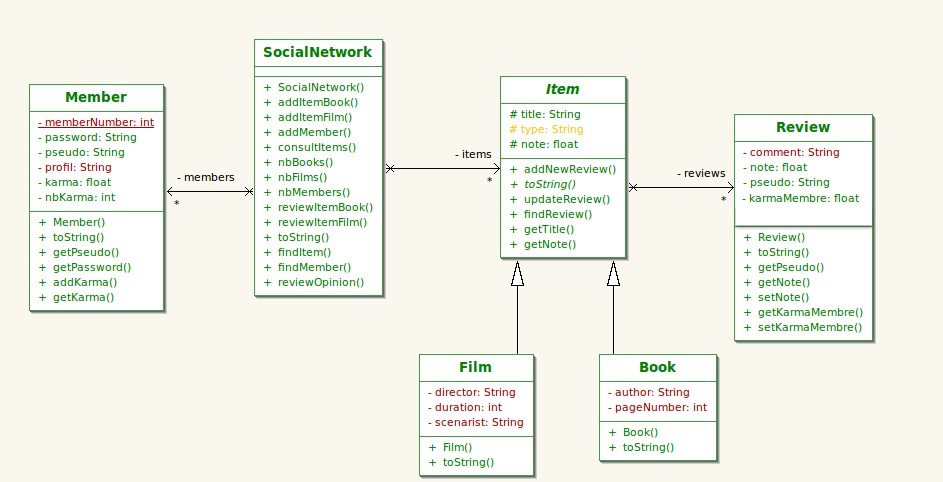
\includegraphics[angle = 90, scale=0.8]{Classe1.jpeg}
\caption{Diagramme général de classes}
\label{fig:diagClasses1}
\end{figure}

\begin{figure}[h]
\centering
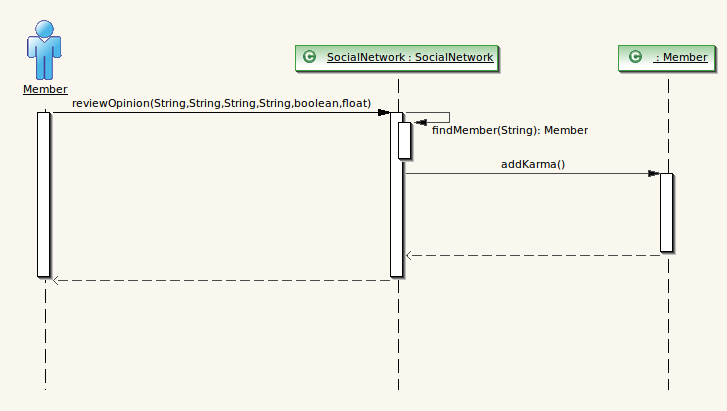
\includegraphics[angle = 90, scale=0.85]{Sequence1.png}
\caption{Diagramme de séquence de reviewOpinion}
\label{fig:diagSeq1}
\end{figure}


\begin{figure}[h]
\centering
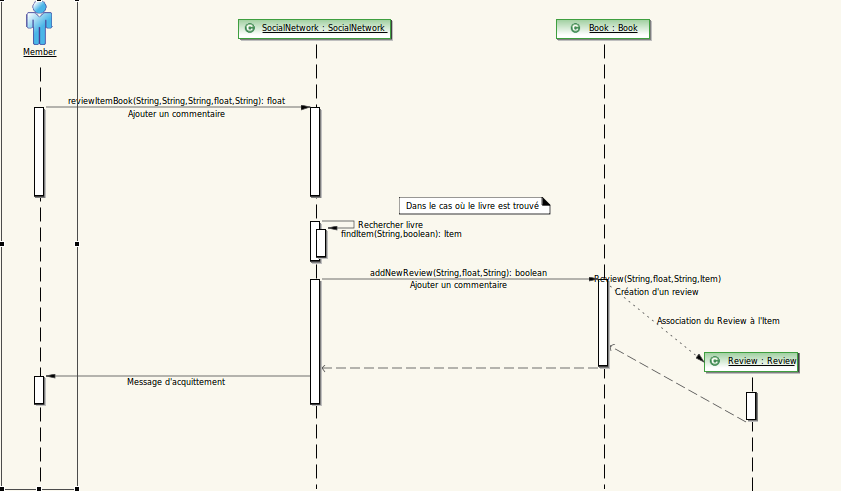
\includegraphics[angle = 90, scale=0.85]{Sequence2.png}
\caption{Diagramme de séquence de reviewItemBook}
\label{fig:diagSeq2}
\end{figure}

\chapter*{Rapport d'audit}
\label{chapter:Rapport d'audit} %Ajout dans la table des matières
\addcontentsline{toc}{chapter}{Rapport d'audit}
Le rapport d'audit effectué par un autre binôme nous a amené à changer notre code. Au total, se sont 8 remarques qui nous ont été faites. 7 d'entre elles concernaient un problème de fond et 1 un problème de forme. Nous avons acceptés 7 remarques pertinentes. La remarque que nous avons refusée n'était qu'une mauvaise compréhension d'un commentaire de test. \\

La remarque de forme était très pertinente. En effet, le problème remonté était que nous utilisions toujours les mêmes conditions pour tester la validité des paramêtres donnés (\emph{pseudo}, \emph{password}, etc). Le copier-coller, rendant la tâche facile, nous à permis de réutiliser les conditions des blocs \emph{if} aisément. Cependant, il est plus claire et efficace de créer des fonctions qui renvoient \emph{true} ou \emph{false} selon un paramêtre donné. Ainsi, s'il faut modifier la manière dont est testé le \emph{password} par exemple, il suffit de modifier la fonction. Toutes les conditions utilisant cette fonction seront donc à jour, contrairement à la méthode que nous avions utilisée.\\

Les autres remarques, bien que pertinentes, n'étaient pas très graves et relevaient la plupart du temps de petits détails.

\chapter*{Rapport de recette}
\label{chapter:Rapport de recette} %Ajout dans la table des matières
\addcontentsline{toc}{chapter}{Rapport de recette}

\begin{tabular}{|p{2.1cm}|p{1.5cm}|p{1.5cm}|p{1.5cm}|p{1.5cm}|p{2cm}|p{2cm}|}
\hline 
Nombre de tests prévus & Tests passés & Tests OK & Tests Non OK & Tests NS & Anomalies majeures & Anomalies mineures \\ 
\hline 
8 & 8 & 8 & 0 & 0 & 0 & 1 \\ 
\hline 
\end{tabular} 

\begin{tabular}{|c|p{4cm}|p{4cm}|p{4cm}|} 
\hline 
Numéro & Identification du test & Résultats & Gravité \\ 
\hline 
1 & Test en environnement <<prestataire>> : avec instructions du fichier <<alire>>. & OK, pas d'erreur, mais il n'est pas possible de tester le lot2 depuis l'IHM & Mineure \\ 
\hline 
2 & TestsInitialisation & ok & RAS \\ 
\hline 
3 & TestsAddMember & ok & RAS \\ 
\hline 
4 & TestsAddItemFilm & ok & RAS \\ 
\hline 
5 & TestsAddItemBook & ok & RAS \\ 
\hline 
6 & TestsReviewItemFilm & ok & RAS \\ 
\hline 
7 & TestsReviewItemBook & ok & RAS \\ 
\hline 
8 & TestsReviewOpinion & ok & RAS \\ 
\hline 
\end{tabular}\\

Lors de cette recette, aucune erreur importante n'a été relevée par le binôme client. Aucune modification n'a donc été apportée. Le fait que nos tests, ainsi que les tests du binôme client, ne relèvent aucune erreur nous permet donc de s'assurer de la conformité de notre livrable par rapport au cahier des charges.

Ci-dessous les fiches de tests du binôme correcteur.

\begin{figure}

\textbf{\begin{center}
Fiche de test N3   
\end{center}} 

\textbf{Objectif du test }: éprouver la méthode addItemFilm sur les cas d'anomalie. 
Vérification de la levée de l'exception BadEntry lors de l'utilisation de AddItemFilm « avec des paramètres d'entrées incorrects ». 
\textbf{Pour rappel }: Les 5 cas de levée de l'exception BadEntry par la méthode addItemFilm prévus dans l'API sont :
\begin{itemize}
	\item	Si le pseudo n’est pas instancié ou a moins de 1 caractère autre que des espaces.
	\item	Si le password n’est pas instancié ou a moins de 4 caractères autres que des leadings or traling blanks.
	\item	Si le titre n’est pas instancié ou a moins de 1 caractère autre que des espaces.
	\item	Si le genre n’est pas instancié.
	\item	Si le réalisateur n’est pas instancié.
	\item	Si le scénariste n’est pas instancié.
	\item	Si la durée n’est pas positive
\end{itemize}

\textbf{Description (scénario) :}
\begin{itemize}
	\item	Instanciation d’un Social Network
	\item	1.1 Utilisation de AddItemFilm avec en paramètre un pseudo non instancié.
	\item	1.2 Utilisation de AddItemFilm avec en paramètre un pseudo ne contenant que des espaces.
	\item	1.3 Utilisation de AddItemFilm avec en paramètre un titre non instancié.
	\item	1.4 Utilisation de AddItemFilm avec en paramètre un titre ne contenant moins d’un caractère autres que des leadings or traling blanks.
	\item	1.5 Utilisation de AddItemFilm avec en paramètre un genre non instancié.
	\item	1.6 Utilisation de AddItemFilm avec en paramètre un réalisateur non instancié.
	\item	1.7 Utilisation de AddItemFilm avec en paramètre un scénariste non instancié.
	\item	1.8 Utilisation de AddItemFilm avec en paramètre une durée négative.
\end{itemize}

\textbf{Résultats attendus :}
Dans les 8 cas d’utilisations de AddItemFilm, l’exception BadEntry doit être levée.
De plus, après la levée de l’exception BadEntry lors de l’utilisation de AddItemFilm, le nombre de films doit rester identique au nombre de Film avant l’utilisation de AddItemFilm.

\textbf{Résultats observés :}

Les 8 cas d'utilisation lèvent bien une exception BadEntry comme prévu, le nombre de films n'a pas été modifié.

\textbf{Conclusion :}

Les tests sont concluants, l'application respecte le CdC.
\caption{Fiche de tests numéro 3}
\end{figure}


\begin{figure}
\textbf{\begin{center}
Fiche de test N4 
\end{center}} 

\textbf{Objectif du test} : éprouver la méthode AddItemFilm sur les cas de fonctionnement standard.

\begin{itemize}
	\item	But principal : Vérification de l’ajout d’un nouvel item de film après l’utilisation de AddItemFilm après un fonctionnement « avec des paramètres d’entrées corrects ».	
	\item	Buts secondaires : 
\begin{itemize}
	\item	Vérification de la levée d’exception NotMember par la méthode AddItemFilm dans tous les cas prévu dans l’API.

	\item	Vérification de la levée d’exception ItemFilmAlreadyExists par la méthode AddItemFilm dans tous les cas prévu dans l’API.
\end{itemize}
\end{itemize}


\textbf{Description (scénario) :}
\begin{itemize}
	\item 	Instanciation d’un Social Network
	\item 	2.1 Utilisation de AddItemFilm pour l’ajout de plusieurs Item « avec des paramètres d’entrées corrects »
	\item 	2.2 Utilisation de AddItemFilm avec en paramètre un pseudo non existant.
	\item 	2.3 Utilisation de AddItemFilm avec en paramètre un couple login/password non cohérent.
	\item  2.4 Utilisation de AddItemFilm avec en paramètre un item film de même titre déjà présent (mais avec des leadings et trailings blanks).
\end{itemize}

\textbf{Résultats attendus :}

L’ajout d’item de Film « avec des paramètres d’entrée corrects » ne doit pas lever d’exception, le nombre d’items de Film après ces ajouts doit avoir augmenté en conséquence.
Dans les 2 utilisations suivantes de AddItemFilm, l’exception NotMember doit être levée.
Dans la dernière utilisation, l’exception ItemFilmAlreadyExists doit être levée.

De plus, après la levée de ces deux exceptions, le nombre d’items de Film doit rester identique au nombre d’items de Film avant l’appel de la fonction AddItemFilm.

\textbf{Résultats observés :}

Les résultats sont en concordance avec ce qui était attendu.

\textbf{Conclusion :}

Le code respecte le CdC.

\caption{Fiche de test numéro 4}
\end{figure}

\begin{figure}
\textbf{\begin{center}
Fiche de test N11  
\end{center}} 
\textbf{Objectif du test :} éprouver la méthode reviewOpinion sur les cas d'anomalie. 

Vérification de la levée de l'exception BadEntry lors de l'utilisation de reviewOpinion « avec des paramètres d'entrées incorrects ». 
Pour rappel : Les 5 cas de levée de l'exception BadEntry par la méthode reviewOpinion prévus dans l'API sont :
\begin{itemize}
	\item Si le pseudo n’est pas instancié ou a moins de 1 caractère autre que des espaces.
	\item 	Si le password n’est pas instancié ou a moins de 4 caractères autres que des leadings or trailing blanks.
	\item 	Si le titre n’est pas instancié ou a moins de 1 caractère autre que des espaces.
	\item 	Si le genre n’est pas instancié.
	\item 	Si le réalisateur n’est pas instancié.
	\item 	Si le scénariste n’est pas instancié.
	\item 	Si la durée n’est pas positive.
\end{itemize}
\textbf{Description (scénario) :}
\begin{itemize}
	\item	Instanciation d’un Social Network
	\item	1.1 Utilisation de ReviewOpinion avec en paramètre un pseudo non instancié.
	\item	1.2 Utilisation de ReviewOpinion avec en paramètre un pseudo ne contenant que des espaces.
	\item	1.3 Utilisation de ReviewOpinion avec en paramètre un titre non instancié.
	\item	1.4 Utilisation de ReviewOpinion avec en paramètre un titre ne contenant moins d’un caractère autres que des leadings or traling blanks.
	\item	1.5 Utilisation de ReviewOpinion avec en paramètre un genre non instancié.
	\item	1.6 Utilisation de ReviewOpinion avec en paramètre un réalisateur non instancié.
	\item	1.7 Utilisation de ReviewOpinion avec en paramètre un scénariste non instancié.
	\item	1.8 Utilisation de ReviewOpinion avec en paramètre une durée négative.
\end{itemize}

\textbf{Résultats attendus :}

Dans les 8 cas d’utilisations de ReviewOpinion, l’exception BadEntry doit être levée.
De plus, après la levée de l’exception BadEntry lors de l’utilisation de ReviewOpinion, le nombre de films doit rester identique au nombre de Film avant l’utilisation de ReviewOpinion.

\textbf{Résultats observés :}

Les exceptions sont levées correctement.

\textbf{Conclusion :}

Le CdC est respecté.

\caption{Fiche de test numéro 11}
\end{figure}


\begin{figure}
\textbf{\begin{center}
Fiche de test N12  
\end{center}} 
\textbf{Objectif du test :} éprouver la méthode reviewOpinion sur les cas de fonctionnement standard. 

\textbf{But principal :} vérification de l'ajout d'une opinion après l'utilisation de reviewOpinion avec des paramètres d'entrée corrects.

\textbf{But secondaire :} vérification des levées des exception NotItem, NotMember.

\textbf{Description (scénario) :}
\begin{itemize}
	\item	Instanciation d’un Social Network
	\item	Utilisation de addMember pour l'ajout de plusieurs membres avec paramètres d'entrées corrects.
	\item	Utilisation de addItemBook pour l'ajout de deux Items Book.
	\item	Utilisation de addItemFilm pour l'ajout d'un Item Film.
	\item	Utilisation de ReviewItemBook pour création d'une opinion sur les deux items Book.
	\item	Utilisation de  ReviewItemFilm pour création d'une opinion sur  l'Item Film.
	\item	1.1 Utilisation de ReviewOpinion avec paramètres d'entrée corrects pour review des trois items crées.
	\item	1.2 Utilisation de ReviewOpinion avec en paramètre un Membre inexistant.
	\item	1.3 Utilisation de ReviewOpinion avec en paramètre un titre d' Item inexistant.
	\item	1.4 Utilisation de ReviewOpinion avec en paramètre un pseudo de « reviewer » inexistant.
\end{itemize}
\textbf{Résultats attendus :}

Dans les 3 derniers cas d’utilisations de ReviewOpinion, les exceptions NotItem et NotMember doivent être levées.
L'utilisation standard de ReviewOpinion doit modifier le karma de l'auteur de la review pour l'item concerné.

\textbf{Résultats observés :}

Les résultats observés sont conformes.

\textbf{Conclusion :}

Le code respecte le CdC.
\caption{Fiche de test numéro 12}
\end{figure}

\begin{figure}
\textbf{\begin{center}
Fiche de test N5
\end{center}}
\textbf{Objectif du test :} éprouver la méthode reviewItemFilm sur les cas d'anomalie. Vérification de la levée de l'exception BadEntry lors de l'utilisation de reviewItemFilm « avec des paramètres d'entrées incorrects ».
\textbf{Pour rappel :} Les 5 cas de levée de l'exception BadEntry par la méthode reviewItemFilm prévus dans l'API sont :  
\begin{itemize}
	\item	Si le pseudo n’est pas instancié ou a moins de 1 caractère autre que des espaces.
	\item	Si le password n’est pas instancié ou a moins de 4 caractères autres que des leadings or traling blanks. 
	\item	Si le titre n’est pas instancié ou a moins de 1 caractère autre que des espaces. 
	\item	Si la note n'est pas comprise entre 0.0 et 5.0 
	\item	Si le commentaire n’est pas instancié. 
\end{itemize}
\textbf{Description (scénario) :}
\begin{itemize}
    \item	Instanciation d’un Social Network 
	\item	Instanciation de trois utilisateurs 
	\item	Instanciation de trois films 
	\item	1.1 Utilisation de reviewItemFilm avec en paramètre un pseudo non instancié. 
	\item	1.2 Utilisation de reviewItemFilm avec en paramètre un pseudo ne contenant que des espaces. 
	\item	1.3 Utilisation de reviewItemFilm avec en paramètre un password non instancié. 
	\item	1.4 Utilisation de reviewItemFilm avec en paramètre un password contenant moins de 4 caractères autres que des leading et trailing blanks. 
	\item	1.5 Utilisation de reviewItemFilm avec en paramètre un titre non instancié. 
	\item	1.6 Utilisation de reviewItemFilm avec en paramètre un titre ne contenant que des espaces . 
	\item	1.7 Utilisation de reviewItemFilm avec en paramètre une note négative 
	\item	1.8 Utilisation de reviewItemFilm avec en paramètre une note supérieure à 5.0 
	\item	1.9 Utilisation de reviewItemFilm avec en paramètre un commentaire non instancié. 
\end{itemize}

\textbf{Résultats attendus : }
Dans les 9 cas d’utilisations de reviewItemFilm, l’exception BadEntry doit être levée. 
De plus, après la levée de l’exception BadEntry lors de l’utilisation de reviewItemFilm, le nombre de films doit rester identique au nombre de Film avant l’utilisation de reviewItemFilm. 

\textbf{Résultats observés : }
Résultats conformes.

\textbf{Conclusion : }
CdC respecté.
\caption{Fiche de test numéro 5}
\end{figure}


\begin{figure}
\textbf{\begin{center}
Fiche de test N6 
\end{center}} 
\textbf{Objectif du test }: éprouver la méthode reviewItemFilm sur les cas de fonctionnement standard. 
\begin{itemize}
	\item	But principal : Vérification de l’ajout ou de la mise à jour d’une opinion concernant l'item film après l’utilisation de reviewItemFilm après un fonctionnement «avec des paramètres d’entrées corrects ». 
	\item	Buts secondaires :  Vérification de la levée d’exception NotMember par la méthode reviewItemFilm dans tous les cas prévus dans l’API. 
	\item \begin{itemize}
	\item Vérification de la levée d’exception NotItem par la méthode reviewItemFilm dans tous les cas prévu dans l’API. 
\end{itemize}		
\end{itemize}
\textbf{Description (scénario) : }
\begin{itemize}
	\item	Instanciation d’un Social Network 
	\item	2.1 Utilisation de reviewItemFilm pour l’ajout de plusieurs opinions « avec des paramètres d’entrées corrects » 
	\item	2.2 Utilisation de reviewItemFilm avec en paramètre un pseudo non existant. 
	\item	2.3 Utilisation de reviewItemFilm avec en paramètre un couple login/password non cohérent. 
	\item	2.4 Utilisation de reviewItemFilm avec en paramètre un item film de titre inexistant. 
\end{itemize}
\textbf{Résultats attendus : }

L’ajout d’une opinion sur un Film « avec des paramètres d’entrées corrects» ne doit pas lever d’exception. La nouvelle opinion saisie constitue la mise à jour de l'opinion. Dans les 2 utilisations suivantes de reviewItemFilm, l’exception NotMember doit être levée. 
Dans la dernière utilisation, l’exception NotItem doit être levée. 
De plus, après la levée de ces deux exceptions, l'opinion du membre concernant l'item film, existante ou pas, doit être identique à l'opinion avant l’appel de la fonction reviewItemFilm. 

\textbf{Résultats observés : }
Les résultats sont conformes.

\textbf{Conclusion : }
Le CdC est respecté.

\caption{Fiche de test numéro 6}
\end{figure}



\chapter*{Bilan}
\label{chapter:Bilan} %Ajout dans la table des matières
\addcontentsline{toc}{chapter}{Bilan}
Le livrable remis du logiciel ToutAvis comprend le lot 1 et 2. Le code est simple et efficace (nombre de lignes de code<1000) tout en respectant toutes les exigences du cahier des charges. Cette simplicité permet également au logiciel de remplir les critères de rendement.

Comme expliqué précedemment, la relecture croisée a été très bénéfique à notre programme. Beaucoup d'améliorations ont été apportées à la suite de ce retour. Il a permis à un autre binôme de donner un nouveau regard sur notre code et de détecter des détails auxquels nous n'avions pas pensé. Ci-dessous, la liste des améliorations apportées à la suite du rapport d'audit:
\begin{itemize}
	\item	Suppression de la méthode getPassword() remplacée par une méthode interne au membre pour respecter l'encapsulation et protéger la donnée.
	\item	Dans reviewOpinion(), ajout d'une vérification pour confirmer que le membre a bien commenté l'item.
	\item	Remplacement des tests pour lever les exceptions par des fonctions qui permettent de mettre à jour très facilement le code. 
	\item	Mise à jour de certains commentaires dans le code pour le rendre plus lisible.
\end{itemize}

La recette n'ayant remonté aucun défaut, il n'y a pas eu de modification ultérieure au rapport de recette.
Le logiciel ToutAvis est donc totalement fonctionnel. Quelques améliorations non-présentes dans le cahier des charges peuvent toute fois encore être ajoutées.

\begin{center}
\begin{tabular}{|c|c|p{6cm}|}
\hline 
Fonction & Pourcentage de validité & Améliorations possibles \\ 
\hline 
addMember & 100\% & RAS \\ 
\hline 
addItemFilm & 100\% & RAS \\ 
\hline 
addItemBook & 100\% & RAS \\ 
\hline 
reviewItemFilm & 100\% & RAS \\ 
\hline 
reviewItemBook & 100\% & RAS \\ 
\hline 
reviewOpinion & 80\% & système de notation à améliorer(un utilisateur peut noter un même membre sur plusieurs commentaires)  \\ 
\hline 
\end{tabular}\\
\end{center}
\begin{center}
\textbf{Figure 10: }Bilan fonctionnel du produit livré
\end{center}

Passons maintenant au bilan non fonctionnel du projet. Pour évaluer le rendement de notre programme,
nous avons codé une classe \emph{TestEfficient} qui permet de mesurer le temps d'exécution des méthodes clés du projet (i.e celles utilisées directement par l'IHM). Ces méthodes sont appelées au sein d'un \emph{SocialNetwork} contenant 500 membres et 5000 items. Ci-dessous un exemple de code écrit :

\begin{figure}[h]
\begin{lstlisting}[caption = Code de rendement d'une fonction]
...
double duree;
//Timer
double start;
start = System.nanoTime();
try{
	sn.addMember("toto", "password", "nouveau membre");
}
catch(BadEntry e)
{
	System.out.println("BadEntry");
}
catch(MemberAlreadyExists e)
{
System.out.println("MemberAlreadyExists");
}
duree = System.nanoTime() - start;
System.out.println("Duree pour ajouter un nouveau membre : " + duree/1000000000 + " secondes\n");
...
\end{lstlisting} 
\begin{center}
{\small Utilisation de System.nanoTime() pour mesurer la durée d'exécution de la méthode \textbf{addMember}}
\end{center}
\end{figure}

\begin{figure}[h]
Les résultats obtenus suivants sont tout-à-fait concluant et respectent le cahier des charges.
\begin{lstlisting}[caption = Resultats obtenus]
Duree pour ajouter un nouveau membre : 8.0896E-5 secondes
Duree pour ajouter un film : 3.88864E-4 secondes
Duree pour ajouter un livre : 0.001121024 secondes
Duree pour rechercher un item : 0.001814016 secondes
Duree pour ajouter un avis sur un Film : 0.00116992 secondes
Duree pour ajouter un avis sur un Book : 0.001432064 secondes
Duree pour ajouter un opinion(karma) a un membre : 0.001236992 secondes
\end{lstlisting}
\end{figure}

\chapter*{Bilan général}
\label{chapter:Bilan général} %Ajout dans la table des matières
\addcontentsline{toc}{chapter}{Bilan général}
Pour dresser un bilan général du travail réalisé, nous pouvons tout d'abord dire que nous avons réussi à s'organiser au sein du binôme pour se répartir au mieu les tâches. De plus, l'utilisation de solution de <<versioning>> (\textbf{GitHub}) à grandement facilité le partage, la mise en commun du code et l'efficacité au sein du binôme.
\begin{quotation}
\textit{- Quels sont les points faibles et les points forts de votre livrable ?}
\end{quotation}


Le livrable que nous proposons est, d'une part, simple à comprendre grâce à une javadoc garnie et, d'autre part, fidèle au cahier des charges grâce notamment à la batterie de tests effectués sur celui-ci. En plus des tests <<classiques>> sur les méthodes et les classes qui vont être utilisées, nous avons effectués des tests de rendement sur l'utilisation de celle-ci. 

\begin{quotation}
\textit{- Si c'était à refaire, que changerions-nous, le cas échéant, dans notre démarche de conception-réalisation ?}
\end{quotation}

Pour reprendre la remarque relevée lors du rapport d'audit, nous pouvons dire qu'une des erreurs que nous avons faite a été de commencer le codage des méthodes trop rapidement. En soit, le premier code proposé n'était pas mauvais, mais il n'était pas correctement structuré. En effet, un temps de réflexion au préalable, sur les fonctions et les conditions qui allaient être appelées fréquement, nous aurait permis de gagner du temps en fin de projet. 

\begin{quotation}
\textit{- Quels sont les avantages et inconvénients trouvés dans la démarche de conception en W ?}
\end{quotation}


La démarche de conception en $W$ nous a permis d'améliorer notre programme comparé à la version initiale. Contrairement à un cycle en $V$, le cycle en $W$ nous a permis d'avoir une vision extérieure sur le travail réalisé. Ces remarques ont été crutiales pour rendre notre code plus facile à modifier et à mettre à jour. Cependant un cycle en spirale aurait permis grâce à un plus grand nombre d'itérations de créer un logiciel plus complexe et robuste. Le principale obstacle qui nous a empêché de travailler de cette manière a été l'investissement en temps nécessaire à l'application d'une telle méthode. 

La conception en $W$ possède quelques avantages, comme par exemple le fait, qu'en suivant ce cycle, nous sommes obligés de passer du temps sur l'analyse et sur la conception. Le temps passé lors de ces deux phases, nous a permit de nous assurer que la phase de réalisation n'allait pas être vaine et que ce que nous allions faire correspondait bien à la demande. De plus, les phases de tests (unitaires et d'intégration) permettent de valider au fur et à mesure les différentes parties du projet.\\

\appendix
\chapter{Fiche de test N3 - addItemFilm}
\textbf{Objectif du test :} éprouver la méthode addItemFilm sur des cas d'anomalie.
Vérification de la levée de BadEntry lors de l’utilisation de addItemFilm avec des paramètres d'entrées incorrects.
Pour rappel, les 7 cas de levée de l'exception BadEntry par cette méthode sont :
\begin{itemize}
\item Si le pseudo n'est pas instancié ou a moins de 1 caractère autre que des espaces
\item Si le password n'est pas instancié ou a moins de 4 caractères autres des leading or trailing blancks
\item Si le titre n'est pas instancié, ou a moins de 1 caractère autre que des espaces
\item Si le genre n'est pas instancié
\item Si le réalisateur n'est pas instancié
\item Si le scénariste n'est pas instancié
\item Si la durée n'est pas positive
\end{itemize}

\textbf{Description (scénario) :}
\begin{itemize}
	\item	Instanciation d'un Social Network
	\item	3.1 : Utilisation de addItemFilm avec en paramètre un pseudo non instancié
	\item	3.2 : Utilisation de addItemFilm avec en paramètre un pseudo avec moins de 1 caractère
	\item	3.3 : Utilisation de addItemFilm avec en paramètre un password pas instancié
	\item	3.4 : Utilisation de addItemFilm avec en paramètre un password de moins de 4 caractères
	\item	3.5 : Utilisation de addItemFilm avec en paramètre un titre non instancié
	\item	3.6 : Utilisation de addItemFilm avec en paramètre un titre de moins de 1 caractère
	\item	3.7 : Utilisation de addItemFilm avec en paramètre un genre non instancié
	\item	3.8 : Utilisation de addItemFilm avec en paramètre un réalisateur non instancié
	\item	3.9 : Utilisation de addItemFilm avec en paramètre un scénariste non instancié
	\item	3.10 : Utilisation de addItemFilm avec en paramètre une durée qui n'est pas positive

\end{itemize}

\textbf{Résultats attendus :}
Dans les 10 cas d'utilisation, l'exception BadEntry doit être levée.
Après la levée d'exception, le nombre d'itemFilm doit rester le même., C'est à dire qu'aucun film ne doit être ajouté.

\textbf{Résultats observés : }
Tests 0/10. Pas d'erreur

\textbf{Conclusion }: RAS

\chapter{Fiche de test N4 - addItemFilm}  

\textbf{Objectif du test : }éprouver la méthode addItemFilm sur des cas de fonctionnement standard.
\begin{itemize}
	\item	But principal : vérification de l'ajout du nouveau film après l'utilisation de addItemFilm avec des paramètres d'entrées corrects.
	\item	Buts secondaires : 
	\begin{itemize}
		\item Vérification de la levée d'exception NotMember par la méthode addItemFilm si le pseudo n'est pas celui d'un membre ou si le pseudo et le password ne correspondent pas.
		\item Vérification de la levée d'exception ItemFilmAlreadyExists par la méthode addItemFilm si un itemFilm existe déjà avec le même titre (indifférent à la casse et aux leadings et trailings blanks)
	\end{itemize}

\end{itemize}

\textbf{Description(scénario) :}
\begin{itemize}
	\item	Instanciation d'un Social Network
	\item	Instanciation de plusieurs Member de test, que si les tests liés à addMember (cf. fiches de test N°1 et N°2) ont été validés
	\item	4.1 : Utilisation de addItemFilm avec des paramètres d'entrées corrects
	\item	4.2 : Utilisation de addItemFilm avec en paramètre un pseudo qui n'est pas celui d'un membre
	\item	4.3 : Utilisation de addItemFilm avec en paramètre un pseudo et un password qui ne correspondent pas
	\item	4.4 : Utilisation de addItemFilm avec en paramètre un titre de film déjà existant

\end{itemize}

\textbf{Résultats attendus :}
	L'ajout d'un ItemFilm avec des paramètres corrects ne doit pas lever d'exception. Le nombre de ItemFilm doit augmenter en conséquence. Pour les deux tests suivants, l'exception NotMember doit être levée. Enfin, pour le dernier test, l'exception ItemFilmAlreadyExists doit être levée. Le nombre de ItemFilm ne doit pas augementer dans ce cas.

\textbf{Résultats observés :}
Tests 0/4. Pas d'erreur

\textbf{Conclusion :} RAS

\chapter{Fiche de test N5 - reviewItemFilm}

\textbf{Objectif du test :} éprouver la méthode reviewItemFilm sur des cas d'anomalie.
Vérification de la levée de BadEntry lors de l’utilisation de reviewItemFilm avec des paramètres d'entrées incorrects.
Pour rappel, les 5 cas de levée de l'exception BadEntry par cette méthode sont :
\begin{itemize}
	\item	Si le pseudo n'est pas instancié ou a moins de 1 caractère autre que des espaces
	\item	Si le password n'est pas instancié ou a moins de 4 caractères autres des leading or trailing blancks
	\item	Si le titre n'est pas instancié, ou a moins de 1 caractère autre que des espaces
	\item	Si la note n’est pas comprise entre 0 et 5
	\item	Si le commentaire n’est pas instancié
\end{itemize}

\textbf{Description (scénario) :}
\begin{itemize}
	\item	Instanciation d'un Social Network
	\item	5.1 : Utilisation de reviewItemFilm avec en paramètre un pseudo non instancié
	\item	5.2 : Utilisation de reviewItemFilm avec en paramètre un pseudo avec moins de 1 caractère
	\item	5.3 : Utilisation de reviewItemFilm  avec en paramètre un password pas instancié
	\item	5.4 : Utilisation de reviewItemFilm avec en paramètre un password de moins de 4 caractères
	\item   5.5 : Utilisation de reviewItemFilm avec en paramètre un titre non instancié
	\item	5.6 : Utilisation de reviewItemFilm avec en paramètre un titre de moins de 1 caractère
	\item	5.7 : Utilisation de reviewItemFilm avec en paramètre une note négative
	\item	5.8 : Utilisation de reviewItemFilm avec en paramètre une note supérieure à 5
	\item	5.9 : Utilisation de reviewItemFilm avec un commentaire non instancié
\end{itemize}

\textbf{Résultats attendus :}
Dans les 8 cas d'utilisation, l'exception BadEntry doit être levée.
Après la levée d'exception, le commentaire ne doit pas être  pris en compte. La note du film ne doit pas être modifiée.

\textbf{Résultats observés :}
Tests 0/9. Pas d'erreur

\textbf{Conclusion :} RAS

\chapter{Fiche de test N6 - reviewItemFilm}    

\textbf{Objectif du test : }éprouver la méthode reviewItemFilm sur des cas de fonctionnement standard.
\begin{itemize}
	\item	But principal : vérification de l'ajout du nouveau commentaire de film après l'utilisation de reviewItemFilm avec des paramètres d'entrées corrects.
	\item	Buts secondaires :
	\begin{itemize}
		\item Vérification de la levée d'exception NotMember par la méthode reviewItemFilm si le pseudo n'est pas celui d'un membre ou si le pseudo et le password ne correspondent pas.
		\item Vérification de la levée d'exception NotItem par la méthode reviewItemFilm si le titre n’est pas le titre d’un film.

	\end{itemize}

\end{itemize}

\textbf{Description (scénario) :}
\begin{itemize}
	\item	Instanciation d'un Social Network
	\item	Instanciation de plusieurs Member de test, que si les tests liés à addMember (cf. fiches de test N°1 et N°2) ont été validés
	\item	6.1 : Utilisation de reviewItemFilm avec en paramètre un pseudo qui n'est pas celui d'un membre 
	\item	6.2 : Utilisation de reviewItemFilm avec en paramètre un pseudo et un password qui ne correspondent pas
	\item	6.3 : Utilisation de reviewItemFilm avec des paramètres corrects
	\item	6.4 : Utilisation de reviewItemFilm avec un titre de film qui n’existe pas
\end{itemize}

\textbf{Résultats attendus :}
	L'ajout d'une review avec des paramètres corrects ne doit pas lever d'exception. Le commentaire doit être pris en compte. Pour les tests 6.1 et 6.2, l'exception NotMember doit être levée. Enfin, pour le dernier test, l'exception NoItem doit être levée. Le commentaire ne doit pas être pris en compte dans ces cas.

\textbf{Résultats observés :}
Tests 0/4. Pas d'erreur

\textbf{Conclusion : }RAS

\chapter{Fiche de test N7 - reviewOpinion}
 
\textbf{Objectif du test : }éprouver la méthode reviewOpinion sur des cas d'anomalie.
Vérification de la levée de BadEntry lors de l’utilisation de reviewOpinion avec des paramètres d'entrées incorrects.
Pour rappel, les 5 cas de levée de l'exception BadEntry par cette méthode sont :
\begin{itemize}
	\item	Si le pseudo n'est pas instancié ou a moins de 1 caractère autre que des espaces
	\item	Si le password n'est pas instancié ou a moins de 4 caractères autres des leading or trailing blancks
	\item	Si le titre n'est pas instancié, ou a moins de 1 caractère autre que des espaces
	\item	Si la note n’est pas comprise entre 0 et 5
	\item	Si le pseudo cible n’est pas instancié, ou a moins de 1 caractère autre que des espaces

\end{itemize}

\textbf{Description (scénario) :}
\begin{itemize}
	\item	Instanciation d'un Social Network
	\item	7.1 : Utilisation de reviewOpinion avec en paramètre un pseudo non instancié
	\item	7.2 : Utilisation de reviewOpinion avec en paramètre un pseudo avec moins de 1 caractère
	\item	7.3 : Utilisation de reviewOpinion avec en paramètre un password pas instancié
	\item	7.4 : Utilisation de reviewOpinion avec en paramètre un password de moins de 4 caractères
	\item	7.5 : Utilisation de reviewOpinion avec en paramètre un titre non instancié
	\item	7.6 : Utilisation de reviewOpinion avec en paramètre un titre de moins de 1 caractère
	\item	7.7 : Utilisation de reviewOpinion avec en paramètre un karma négatif
	\item	7.8 : Utilisation de reviewOpinion avec en paramètre un karma supérieur à 5
	\item	7.9 : Utilisation de reviewOpinion avec en paramètre un pseudo cible non instancié
	\item	7.10 : Utilisation de reviewOpinion avec en paramètre un pseudo cible avec moins de 1 caractère
\end{itemize}

\textbf{Résultats attendus :}
Dans les 1er cas d'utilisation, l'exception BadEntry doit être levée.
Après la levée d'exception, l'opinion ne doit pas être prise en compte.Le karma du membre ne doit pas être modifié.

\textbf{Résultats observés :}
Tests 0/10. Pas d'erreur
\textbf{Conclusion : }RAS

\chapter{Fiche de test N8 - reviewOpinion}    

\textbf{Objectif du test :} éprouver la méthode reviewOpinion sur des cas de fonctionnement standard.
\begin{itemize}
	\item	But principal : vérification de l'ajout d'une opinion sur un membre après l'utilisation de reviewOpinion avec des paramètres d'entrées corrects.
	\item	Buts secondaires :
	\begin{itemize}
		\item	Vérification de la levée d'exception NotMember par la méthode reviewOpinion si le pseudo n'est pas celui d'un membre ou si le pseudo et le password ne correspondent pas.
       \item    Vérification de la levée d'exception NotItem par la méthode reviewOpinion si le titre n’est pas dans le SocialNetwork.
	   \item 	Vérification de la levée d'exception SameMember par la méthode reviewOpinion si les 2 pseudos en paramètre sont les mêmes.

	\end{itemize}

\end{itemize}

\textbf{Description (scénario) :}
\begin{itemize}
	\item	Instanciation d'un Social Network
	\item	Instanciation de plusieurs Member de test, que si les tests liés à addMember (cf. fiches de test N°1 et N°2) ont été validés
	\item	8.1 : Utilisation de reviewOpinion avec en paramètre un pseudo qui n'est pas celui d'un membre 
	\item	8.2 : Utilisation de reviewOpinion avec en paramètre un pseudo et un password qui ne correspondent pas
	\item	8.3 : Utilisation de reviewOpinion avec des paramètres corrects
	\item	8.4 : Utilisation de reviewOpinion avec deux pseudos identiques
	\item	8.5 : Utilisation de reviewOpinion avec un titre de film qui n’existe pas
	\item	8.6 : Utilisation de reviewOpinion avec un titre de livre mais bookOrNot faux 

\end{itemize}

\textbf{Résultats attendus :}
	L'ajout d'une review avec des paramètres corrects ne doit pas lever d'exception. L'opinion doit être prise en compte. Pour les tests 8.1 et 8.2, l'exception NotMember doit être levée. Pour le test 8.4, l'exception SameMember doit être levée. Enfin, pour les derniers tests, l'exception NoItem doit être levée. L'opinion ne doit pas être prise en compte dans ces cas.

\textbf{Résultats observés :}
Tests 0/6. Pas d'erreur

\textbf{Conclusion :}RAS
\end{document}